%%%%%%%%%%%%%%%%%%%%%%%%%%%%%%%%%%%%%%%%%
% Masters/Doctoral Thesis 
% LaTeX Template
% Version 2.5 (27/8/17)
%
% This template was downloaded from:
% http://www.LaTeXTemplates.com
%
% Version 2.x major modifications by:
% Vel (vel@latextemplates.com)
%
% This template is based on a template by:
% Steve Gunn (http://users.ecs.soton.ac.uk/srg/softwaretools/document/templates/)
% Sunil Patel (http://www.sunilpatel.co.uk/thesis-template/)
%
% Template license:
% CC BY-NC-SA 3.0 (http://creativecommons.org/licenses/by-nc-sa/3.0/)
%
%%%%%%%%%%%%%%%%%%%%%%%%%%%%%%%%%%%%%%%%%

%----------------------------------------------------------------------------------------
%	PACKAGES AND OTHER DOCUMENT CONFIGURATIONS
%----------------------------------------------------------------------------------------

\documentclass[
11pt, % The default document font size, options: 10pt, 11pt, 12pt
%oneside, % Two side (alternating margins) for binding by default, uncomment to switch to one side
english, % ngerman for German
singlespacing, % Single line spacing, alternatives: onehalfspacing or doublespacing
%draft, % Uncomment to enable draft mode (no pictures, no links, overfull hboxes indicated)
%nolistspacing, % If the document is onehalfspacing or doublespacing, uncomment this to set spacing in lists to single
%liststotoc, % Uncomment to add the list of figures/tables/etc to the table of contents
%toctotoc, % Uncomment to add the main table of contents to the table of contents
%parskip, % Uncomment to add space between paragraphs
%nohyperref, % Uncomment to not load the hyperref package
headsepline, % Uncomment to get a line under the header
%chapterinoneline, % Uncomment to place the chapter title next to the number on one line
%consistentlayout, % Uncomment to change the layout of the declaration, abstract and acknowledgements pages to match the default layout
]{MastersDoctoralThesis} % The class file specifying the document structure

\usepackage[utf8]{inputenc} % Required for inputting international characters
\usepackage[T1]{fontenc} % Output font encoding for international characters

\usepackage{amsmath}
\usepackage{amssymb}
\usepackage{mathrsfs}
\usepackage{subcaption}

\usepackage{mathpazo} % Use the Palatino font by default

%\usepackage[backend=bibtex,style=authoryear,natbib=true]{biblatex} % Use the bibtex backend with the authoryear citation style (which resembles APA)
\usepackage[backend=bibtex,style=numeric,natbib=true]{biblatex} % Use the bibtex backend with the number citation style

\addbibresource{example.bib} % The filename of the bibliography

\usepackage[autostyle=true]{csquotes} % Required to generate language-dependent quotes in the bibliography

\defbibheading{secbib}[References]{%
  \section*{#1}%
  \markboth{#1}{#1}}

%----------------------------------------------------------------------------------------
%	MARGIN SETTINGS
%----------------------------------------------------------------------------------------

\geometry{
	paper=a4paper, % Change to letterpaper for US letter
	inner=1.5cm, % Inner margin
	outer=1.8cm, % Outer margin
	bindingoffset=.5cm, % Binding offset
	top=1.5cm, % Top margin
	bottom=1.5cm, % Bottom margin
	%showframe, % Uncomment to show how the type block is set on the page
}


%----------------------------------------------------------------------------------------
%	THESIS INFORMATION
%----------------------------------------------------------------------------------------

\thesistitle[Linearized General Relativity in Hyperboloidal Coordinates]{Linearized General Relativity in Hyperboloidal Coordinates} % Your thesis title, this is used in the title and abstract, print it elsewhere with \ttitle
\supervisor{David Hilditch} % Your supervisor's name, this is used in the title page, print it elsewhere with \supname
\examiner{} % Your examiner's name, this is not currently used anywhere in the template, print it elsewhere with \examname
\degree{Master in Physics Engineering} % Your degree name, this is used in the title page and abstract, print it elsewhere with \degreename
\author{Filipe Ficalho} % Your name, this is used in the title page and abstract, print it elsewhere with \authorname
\addresses{} % Your address, this is not currently used anywhere in the template, print it elsewhere with \addressname

\subject{Numerical Relativity} % Your subject area, this is not currently used anywhere in the template, print it elsewhere with \subjectname
\keywords{} % Keywords for your thesis, this is not currently used anywhere in the template, print it elsewhere with \keywordnames
\university{\href{http://tecnico.ulisboa.pt}{Instituto Superior T\'ecnico}} % Your university's name and URL, this is used in the title page and abstract, print it elsewhere with \univname
\department{\href{http://department.university.com}{CENTRA}} % Your department's name and URL, this is used in the title page and abstract, print it elsewhere with \deptname
\group{\href{http://researchgroup.university.com}{GRIT}} % Your research group's name and URL, this is used in the title page, print it elsewhere with \groupname
\faculty{\href{http://faculty.university.com}{Faculty Name}} % Your faculty's name and URL, this is used in the title page and abstract, print it elsewhere with \facname

\AtBeginDocument{
\hypersetup{pdftitle=\ttitle} % Set the PDF's title to your title
\hypersetup{pdfauthor=\authorname} % Set the PDF's author to your name
\hypersetup{pdfkeywords=\keywordnames} % Set the PDF's keywords to your keywords
}

\begin{document}

\pagestyle{plain} % Default to the plain heading style until the thesis style is called for the body content

%----------------------------------------------------------------------------------------
%	TITLE PAGE
%----------------------------------------------------------------------------------------

\begin{titlepage}

\begin{minipage}[t]{0.4\textwidth}
\begin{flushleft} 
\vspace{0pt}
\hspace{-1cm}

\includegraphics[scale=0.25]{Images/logo.pdf}
\end{flushleft}
\end{minipage}
\hfill
\begin{minipage}[t]{0.41\textwidth}
\begin{flushright} 
\vspace{0pt}
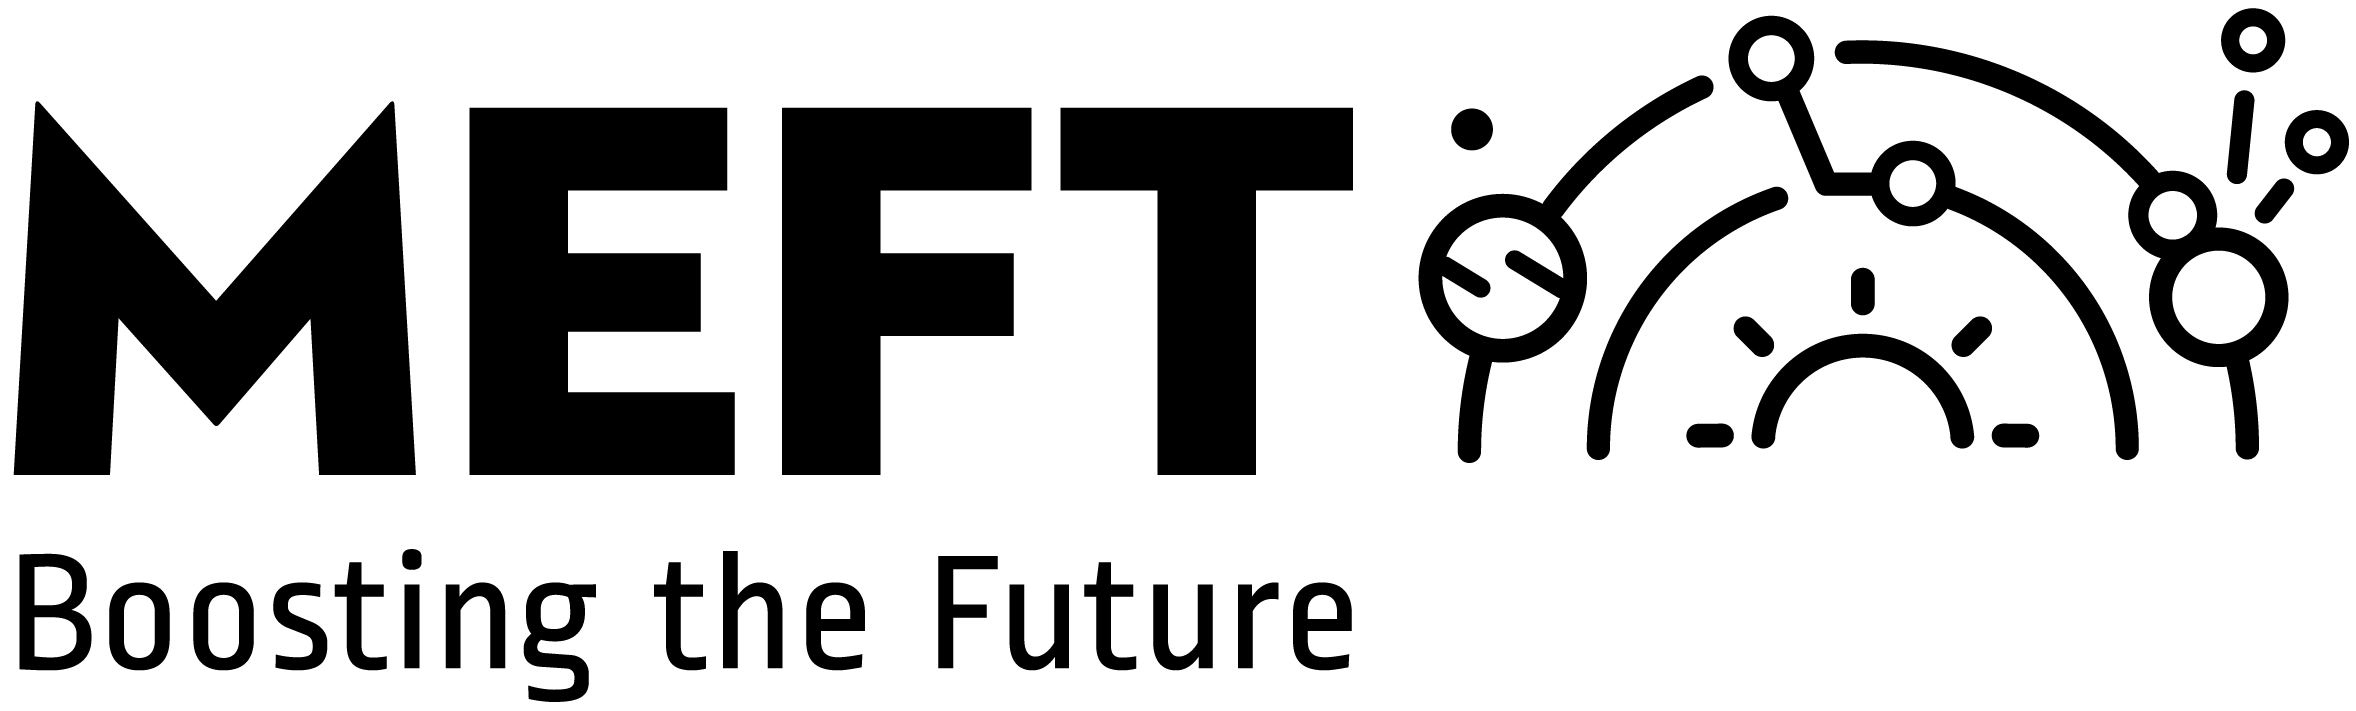
\includegraphics[scale=0.08]{Images/Logo-MEFT_Hor.png}
\end{flushright}
\end{minipage}

\begin{center}

\vspace*{.06\textheight}
{\scshape\LARGE \univname\par}\vspace{1.5cm} % University name
\textsc{\Large Projecto MEFT}\\[0.5cm] % Thesis type

\HRule \\[0.4cm] % Horizontal line
{\huge \bfseries \ttitle\par}\vspace{0.4cm} % Thesis title
\HRule \\[1.5cm] % Horizontal line
 
\begin{minipage}[t]{0.4\textwidth}
\begin{flushleft} \large
\emph{Author:}\\
{\authorname} % Author name
\end{flushleft}
\end{minipage}
\begin{minipage}[t]{0.4\textwidth}
\begin{flushright} \large
\emph{Supervisor:} \\
{\supname} % Supervisor name
\end{flushright}
\end{minipage}\\[3cm]
 
\vfill

\large \textit{Research work performed for the \degreename}\\[0.3cm] % University requirement text
\textit{at}\\[0.4cm]
\groupname\\\deptname\\[2cm] % Research group name and department name
 
\vfill

{\small \today}\\[4cm] % Date
%\includegraphics{Logo} % University/department logo - uncomment to place it
 
\vfill
\end{center}
\end{titlepage}


%----------------------------------------------------------------------------------------
%	THESIS CONTENT - CHAPTERS
%----------------------------------------------------------------------------------------

\pagestyle{review} 


%----------------------------------------------------------------------------------------
%	INTRODUCTION
%----------------------------------------------------------------------------------------

\section{Introduction}
When studying gravitational waves, we must be mindful that gravitational wave sources (like black hole mergers, neutron stars, etc.) are billions of light years away from Earth. From the point of view of an observer on Earth, this distance is so vast that it can be approximated as being at infinity. This distance, however, is not sufficiently far away to require accounting for the cosmological constant, allowing us to model spacetime as asymptotically flat. Thus, we are interested in studying the behavior of the gravitational fields at null infinity, $\mathscr{I}$.

To do so, we may perform a conformal compactification of the spacetime, which brings $\mathscr{I}$ to a finite distance on our computational grid. This is done by working in the hyperboloidal coordinate system.

\subsection{Hyperboloidal Coordinates}

The hyperboloidal coordinate system, as previously mentioned, maps our previously unbonded domain to a finite one by introducing new time and radial coordinates $(t,r)$, which are related to the spherical coordinates of Minkowski spacetime $(T,R)$ by the transformations
%
\begin{equation}
    \begin{array}{l c r} 
        t = T - H(R) & \qquad\qquad\qquad & R = \frac{r}{\Omega(r)} \; ,
    \end{array} \; 
\end{equation}
%
where $H(R)$ is called the height function and $\Omega(r)$ is called the compress function \cite{hilditch2016evolutionhyperboloidaldatadual,Zengino_lu_2011}, which give rize to the Jacobian matrix:
%
\begin{equation}
    \left(J^{Hyp}\right)_{\alpha'}^{\ \ \beta} = 
    \begin{pmatrix}
        1 & -H'(r) & 0 & 0 \\
        0 & \frac{L(r)}{\Omega^2(r)} & 0 & 0 \\
        0 & 0 & 1 & 0 \\
        0 & 0 & 0 & 1
    \end{pmatrix} \; ,
\end{equation}
%
where $H'(r)$ denotes the derivative of the height function with respect to $R$ written as a function of $r$, and $L(r)$ is defined as
%
\begin{equation}
    L(r) \equiv \Omega(r) - r \, \partial_r \Omega(r) \; .
\end{equation}

This coordinate system is advantageous because it allows us to do the desired compactification while maintaining the characteristic speed of outgoing waves finite. Additionally, we can choose the height and compress functions so that the outgoing light speed is constant, which we can observe in figure \ref{fig:Good_Speeds} for a specific choice of the height and compress functions \cite{hilditch2016evolutionhyperboloidaldatadual}. In contrast, this coordinate system makes incoming waves hard to resolve. 

\begin{figure}[h]
    \centering
    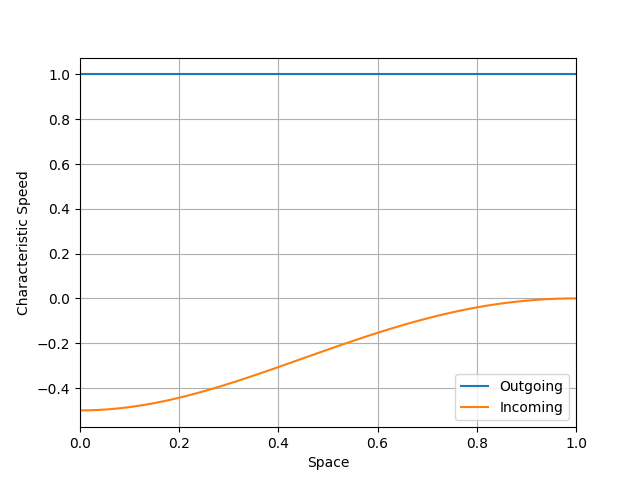
\includegraphics[width=0.5\textwidth]{Images/Good_Speeds.png}
    \caption{Characteristic speeds of the wave equation in hyperboloidal coordinates with $H(R) = \frac{2 R^2 + S^2 - \sqrt{4 R^2 S^2 + S^4}}{2R}$, $\Omega(r) = 1 - \frac{r^2}{S^2}$ and $S = 1$ for outgoing and incoming waves.}
    \label{fig:Good_Speeds}
\end{figure}

Throughout this work, we will sacrifice this very relevant property in exchange for ease of manipulation of the expressions since the goal of this introductory work to the subject is to get accustomed to the coordinate system. The height and compress functions that will used throughout this work are
%
\begin{equation}
    \begin{array}{l c r}
        H(R) = \sqrt{S^2+R^2} & \qquad\qquad\qquad & \Omega(r) = \frac{1}{2} \left(1 - \frac{r^2}{S^2}\right)
    \end{array} \; ,
\end{equation}
%
where $S$ is a constant that determines the size of the compactified domain, which we can choose arbitrarily. To make our domains range from -1 to 1 in the generic case and from 0 to 1 in the spherically symmetric case, we will set $S=1$. As a consequence of our previous choices, we also have
%
\begin{equation}
    \begin{array}{l c r}
        H'(r) = \frac{2 \, r \, S}{S^2 + r^2} & \qquad\qquad\qquad & L(r) = \frac{1}{2} \left(1 + \frac{r^2}{S^2}\right) \; .
    \end{array}
\end{equation}

For this choice of functions, we still have that the incoming light speed decreases as it reaches $\mathscr{I}$. However, we don't have a constant outgoing propagation speed, shown in figure \ref{fig:Bad_Speeds}. The only implication this choice will have in our results is that the wave will take longer to reach $\mathscr{I}$ and will be slightly distorted, which is not problematic since our purpose is to ensure the code converges smoothly toward the solution.

\begin{figure}[h]
    \centering
    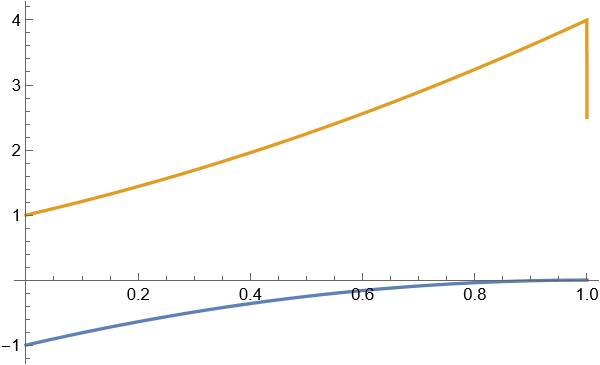
\includegraphics[width=0.5\textwidth]{Images/Bad_Speeds.png}
    \caption{Characteristic speeds of the wave equation in hyperboloidal coordinates with $H(R) = \sqrt{S^2+R^2}$, $\Omega(r) = \frac{1}{2} \left(1 - \frac{r^2}{S^2}\right)$ and $S = 1$ for outgoing and incoming waves.}
    \label{fig:Bad_Speeds}
\end{figure}

\subsection{Computational Setup}

This work is a continuation of my previous work on numerical relativity. As such, the framework used here is the same as the one used there (described in \cite{Ficalho_2023}), with the addition of truncation error matching for the derivatives, interpolation at the boundaries, and the Evans Method for regularization at the origin.

\subsubsection{Truncation Error Matching}

Truncation error matching is a technique used to improve the accuracy of the numerical solution by matching the truncation error of the finite difference scheme used on the boundaries to the truncation error of the one used in the interior of our computational domain. This matching uses a one-sided finite difference scheme on the boundaries such that the leading order error term is the same as the one used in the interior.

In our framework, to approximate the first derivative of a field $\psi$ at an interior point $i$ (writing the leading order error term explicitly), we use 
%
\begin{equation}
    \psi'_i = \frac{\psi_{i+1} - \psi_{i-1}}{2h} - \frac{h^2}{6} \psi'''_i + ...\; ,
\end{equation}
%
where $\psi_{i+1}$ and $\psi_{i-1}$ are the values of the field $\psi$ at the points $i+1$ and $i-1$ respectively, and $h$ is the grid spacing. \cite{Pretorius_2002,Gautam_2021}

To match this leading order term of the error at the left and right boundary points, respectively, we use
%
\begin{equation}
    \psi'_i = \frac{\psi_{i+3} - 4 \psi_{i+2} + 7 \psi_{i+1} - 4 \psi_{i}}{2h} - \frac{h^2}{6} \psi'''_i + ...\;
\end{equation}
%
\begin{equation}
    \psi'_i = \frac{4 \psi_{i} - 7 \psi_{i-1} + 4 \psi_{i-2} - \psi_{i-3}}{2h} - \frac{h^2}{6} \psi'''_i + ...\;
\end{equation}


\subsubsection{Extrapolation at the Boundaries}

Since we are interested in evolving the fields at null infinity, we must choose a boundary condition that allows the fields to propagate out of our computational domain. To do so, we use extrapolation at the outer boundaries of our computational domain to fill the ghost points in those regions. We calculate the value of our fields at the ghost points using
%
\begin{equation}
    \psi_i = 4 \psi_{i-1} - 6 \psi_{i-2} + 4 \psi_{i-3} - \psi_{i-4} \; ,
\end{equation}
%
where $\psi_i$ is the value of the field at the ghost point $i$, and $\psi_{i-1}$, $\psi_{i-2}$, $\psi_{i-3}$ and $\psi_{i-4}$ are the values of the field at the points $i-1$, $i-2$, $i-3$ and $i-4$ respectively.

\subsubsection{Evans Method}
When dealing with operators like the Laplacian in spherical coordinates, we find some formal singularities, like terms where the coefficients are inversely proportional to the radial coordinate, that we must remove for our code to work. To remove those singularities, we can apply the Evans Method. This method involves rewriting the singular terms as a different differential operator, called the Evans operator, which we can evaluate at the grid points. We define this operator as
%
\begin{equation}
    \partial_r \psi + \frac{p}{r}\psi = (p+1) \frac{d(r^p \psi)}{dr^{p+1}}\;,
\end{equation}
%
where $p$ is a constant. This operator can be expressed in terms of the grid points as 
%
\begin{equation}
    (p+1) \frac{d(r^p \psi)}{dr^{p+1}}=(\tilde{D}\psi)_i = (p+1)\frac{r^p_{i+1}\psi_{i+1}-r^p_{i-1}\psi_{i-1}}{r^{p+1}_{i+1}-r^{p+1}_{i-1}}\;,
\end{equation}
%
where the subscripts $i+1$ and $i-1$ denote the grid points $i+1$ and $i-1$ respectively. \cite{Evans_1984}
\newpage

%----------------------------------------------------------------------------------------
%	WAVE EQUATION IN 1+1 DIMENSIONS
%----------------------------------------------------------------------------------------

\section{Wave Equation in 1+1 Dimensions}
We start by considering the wave equation in 1+1 dimensions

\begin{equation}
    \Box \psi \equiv - \partial_T^2 \psi + \partial_X^2  \psi = 0 \;.
\end{equation}

From my previous work on the subject \cite{}, we concluded that we should use systems of equations that are first order both in space and in time, since the second order in space and first order in time scheme proved to be problematic. Thus, we proceed to do a first order reduction of the wave equation by defining $\Pi \equiv -\partial_T \psi$, obtaining

\begin{equation}
    \left\{ \begin{array}{l} 
        \partial_T \psi = - \Pi \\ 
        \partial_T \Pi = -\partial_{\underline{i}} \partial^{\underline{i}} \psi 
    \end{array} \right. \; .
\end{equation}

We can add an additional constraint $C_{\underline{i}} = \partial_{\underline{i}} \psi - \Phi_{\underline{i}} \overset{!}{=} 0$ to our system of equations, to which small violations could be allowed. Using the time derivative of this constraint as an evolution equation for $\Phi$ and expressing the small violation of this constraint as $\gamma_2 C_{\underline{i}}$, where $\gamma_2$ is a small parameter corresponding to the allowed violation, we get

\begin{equation}
    \left\{ \begin{array}{l} 
        \partial_T \psi = - \Pi \\ 
        \partial_T \Phi = - \partial_X \Pi + \gamma_2 \, \partial_X \psi - \gamma_2 \, \Phi\\
        \partial_T \Pi = -\partial_X \Phi
    \end{array} \right. \; .
\end{equation}

We then proceed to make a coordinate change from inertial Minkowski coordinates to hyperboloidal coordinates. Addicionally, even though we could allow for small violations of our constraint, we will not. Thus, we set $\gamma_2 = 0$, obtaining the final form of our system of equations:

\begin{equation}
    \left\{ \begin{array}{l} 
        \partial_t \psi = - \Pi \\ 
        \partial_t \Phi = \mathcal{A} \, \left( H' \, \partial_x \Phi + \partial_x \Pi \right)\\
        \partial_t \Pi = \mathcal{A} \, \left( H' \, \partial_x \Pi + \partial_x \Phi \right)
    \end{array} \right. \; ,
\end{equation}
where we defined $\mathcal{A}(x) =\frac{\Omega^2(x)}{L(x)(H'^{\,2}(x)-1)}$, and dropped the explicit dependences on $x$ to simplify the notation.

We can now solve this system of equations using the aforementioned code, using truncation error matching for the derivatives on the boundaries and turning off the artificial dissipation on those points. Using that framework and giving the initial conditions
\begin{equation}
    \begin{array}{c c c c}
        \psi(0,x) = A \, e^{-C \, x^2/2} \; , & \Phi(0,x) = - A \,C \, x \, \frac{\Omega^2(x)}{L(x)} \, e^{-C \, x^2/2} & \text{and} & \Pi(0,x) = 0
    \end{array} \; ,
    \label{eq:compact_wave_equation-2nd_order_initial_conditions}
\end{equation}
with $A = 1.0$ and $C = 100$, we obtain the evolution present in figure \ref{fig:compact_wave_equation-2nd_order}. In that evolution, it is noticeable that after the wave leaves the grid, we are left with a permanent negative displacement on our field. Even though this result is counterintuitive, it was proven in \cite{} to be correct.

\begin{figure}[h]
    \centering
    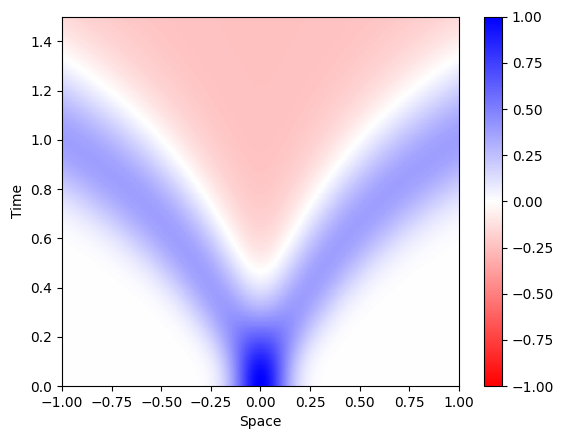
\includegraphics[width=0.5\textwidth]{Images/Wave_Equation_1+1-Solution.png}
    \caption{Evolution of the wave equation in 1+1 dimensions using hyperboloidal coordinates with the initial conditions given in equation \eqref{eq:compact_wave_equation-2nd_order_initial_conditions}.}
    \label{fig:compact_wave_equation-2nd_order}
\end{figure}

Doing a norm convergence test (using the $L^2$ norm), we obtain a clean second order convergence during the whole evolution, as can be seen for $\psi$ in the left of figure \ref{fig:compact_wave_equation-2nd_order-convergence}. We can also see that these results stay promising up until $\mathscr{I}$ through the pointwise convergence at that point, represented in the right of figure \ref{fig:compact_wave_equation-2nd_order-convergence}.

\begin{figure}[h]
    \centering
    \begin{subfigure}[b]{0.45\textwidth}
        \centering
        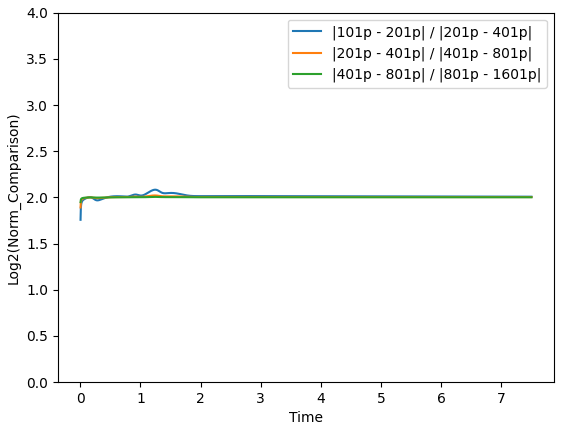
\includegraphics[width=\textwidth]{Images/Wave_Equation_1+1-Norm.png}
    \end{subfigure}
    \hfill
    \begin{subfigure}[b]{0.45\textwidth}
        \centering
        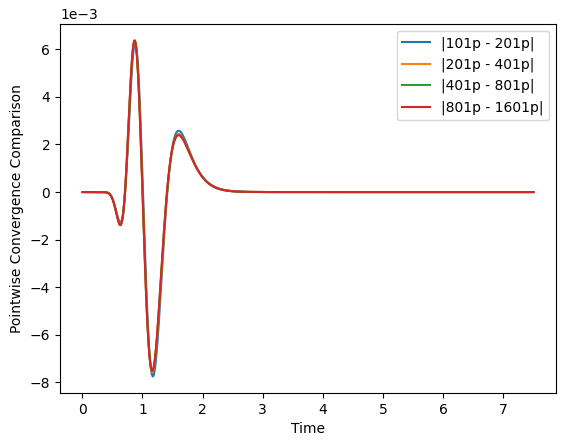
\includegraphics[width=\textwidth]{Images/Wave_Equation_1+1-Pointwise.png}
    \end{subfigure}
    \caption{Convergence tests of the obtained evolutions for the wave equation in 1+1 dimensions using hyperboloidal coordinates. On the left, we have the $L^2$ norm convergence, and on the right, we have the pointwise convergence at $\mathscr{I}$.}
    \label{fig:compact_wave_equation-2nd_order-convergence}
\end{figure}



%----------------------------------------------------------------------------------------
%	WAVE EQUATION IN 3+1 DIMENSIONS WITH SPHERICAL SYMMETRY
%----------------------------------------------------------------------------------------

\section{Wave Equation in 3+1 Dimensions With Spherical Symmetry}
Now, let us consider the wave equation in 3+1 dimensions with spherical symmetry
\begin{equation}
    \Box \psi \equiv - \partial_T^2 \psi + \frac{1}{R^2} \partial_R\left( R^2 \partial_R \psi\right) = 0 \;.
\end{equation}

Since $\psi$ is a solution to this equation, it will decay at a rate of $1/R$, which is a problem because we want to know how our field behaves at $\mathscr{I}$. Thus, we need to renormalize this field in such a way that it does not vanish at infinity. With this in mind, let us define a new field $\Psi$ such that
$$\Psi \equiv \chi \, \psi \; ,$$
where we will take $\chi = \sqrt{1+R^2}$.

Applying that transformation to the wave equation, it becomes

\begin{equation}
    \partial_T^2 \Psi = \partial_R^2\Psi + \frac{2}{R(R^2+1)} \partial_R\Psi - \frac{3}{(R^2+1)^2} \Psi \;,
\end{equation}
%
to which we can apply a first order reduction, obtaining

\begin{equation}
    \left\{ \begin{array}{l} 
        \partial_T \Psi = - \Pi \\ 
        \partial_T \Phi = - \partial_R \Pi + \gamma_2 \partial_R \Psi - \gamma_2\Phi\\
        \partial_T \Pi = - \partial_R \Phi - \frac{2}{R(R^2+1)}\Phi + \frac{3}{(R^2+1)^2} \Psi
    \end{array} \right. \; .
\end{equation}

Doing a coordinate change from inertial Minkowski coordinates to hyperboloidal coordinates and setting $\gamma_2 = 0$ as we did previously, we get

\begin{equation}
    \left\{ \begin{array}{l} 
        \partial_T \Psi = - \Pi \\ 
        \partial_T \Phi = \mathcal{B}\left((r^2 + \Omega^2)^2 \left(H' \partial_r \Phi + \partial_r\Pi\right) + H' L \Omega \left( 2r\Phi - 3 \Omega \Psi + 2 r^{-1} \Omega^2 \Phi\right)\right)\\
        \partial_T \Pi = \mathcal{B}\left((r^2 + \Omega^2)^2 \left(\partial_r \Phi + H' \partial_r\Pi\right) + L \Omega \left( 2r\Phi - 3 \Omega \Psi + 2 r^{-1} \Omega^2 \Phi\right)\right)
    \end{array} \right. \; ,
\end{equation}
where we defined $\mathcal{B}= \frac{\Omega^2}{L(H'^{\,2}-1)(r^2 + \Omega^2)^2}$. 

We can see that in our evolution equations for $\Phi$ and for $\Pi$, we have a term that is formally singular, to which we will need to apply the Evans method. For that, we rewrite those evolution equations, obtaining
\begin{equation}
    \left\{ \begin{array}{l} 
        \partial_T \Psi = - \Pi \\ 
        \partial_T \Phi = \mathcal{B}\left((r^2 + \Omega^2)^2 \left(H' \partial_r \Phi + \partial_r\Pi\right) + H' L \Omega \left( 2r\Phi - 3 \Omega \Psi - \Omega^2 \partial_r \Phi\right) + H' L\Omega^3\left( \partial_r \Phi + 2 r^{-1}\Phi\right) \right)\\
        \partial_T \Pi = \mathcal{B}\left((r^2 + \Omega^2)^2 \left(\partial_r \Phi + H' \partial_r\Pi\right) + L \Omega \left( 2r\Phi - 3 \Omega \Psi - \Omega^2 \partial_r\Phi \right) + L \Omega^3\left( \partial_r \Phi + 2 r^{-1}\Phi \right) \right)
    \end{array} \right. \; ,
\end{equation}
%
where it is easy to see that we can apply the Evans method to the last terms in parenthesis.

Imposing the parity of each field at the origin and doing extrapolation at $\mathscr{I}$ (instead of truncation error matching that we used before) as our boundary conditions and using the initial data
\begin{equation}
    \begin{array}{c c c c}
        \psi(0,r) = A \, e^{-C \, r^2/2} \; , & \Phi(0,r) = - A \,C \, r \, \frac{\Omega^2(r)}{L(r)} \, e^{-C \, r^2/2} & \text{and} & \Pi(0,r) = 0
        \end{array} \; ,
\end{equation}
with $A = 1.0$ and $C = 100$, we obtain the evolution represented in figure \ref{fig:spherical_compact_wave_equation-2nd_order}.

\begin{figure}[h]
    \centering
    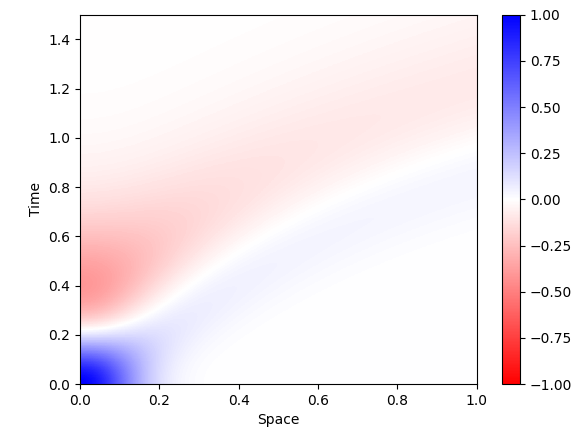
\includegraphics[width=0.5\textwidth]{Images/Wave_Equation_3+1_Spherical-Solution.png}
    \caption{Evolution of the wave equation in 3+1 dimensions with spherical symmetry using hyperboloidal coordinates with the initial conditions given in equation \eqref{eq:compact_wave_equation-2nd_order_initial_conditions}.}
    \label{fig:spherical_compact_wave_equation-2nd_order}
\end{figure}

Similarly to before, we obtain a clean second order convergence during the whole evolution, as can be seen for $\psi$ in the left of figure \ref{fig:spherical_compact_wave_equation-2nd_order-convergence}. Addicionally, we still have very good pointwise convergence at $\mathscr{I}$, as can be seen in the right of figure \ref{fig:spherical_compact_wave_equation-2nd_order-convergence}. Despite the fact that these results are already very good, they could be further improved by doing truncation error matching at the outer boundary instead of the extrapolation that was used.

\begin{figure}[h]
    \centering
    \begin{subfigure}[b]{0.45\textwidth}
        \centering
        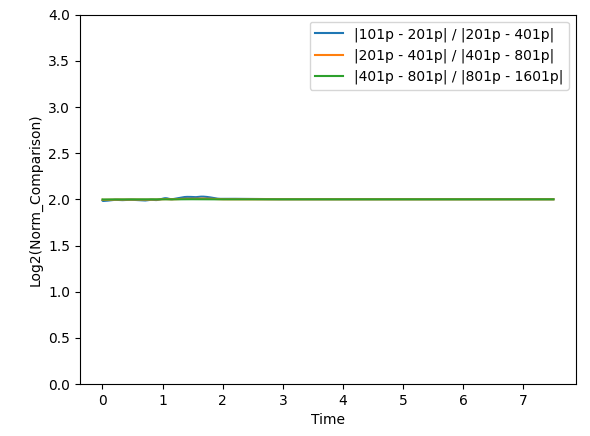
\includegraphics[width=\textwidth]{Images/Wave_Equation_3+1_Spherical-Norm.png}
    \end{subfigure}
    \hfill
    \begin{subfigure}[b]{0.45\textwidth}
        \centering
        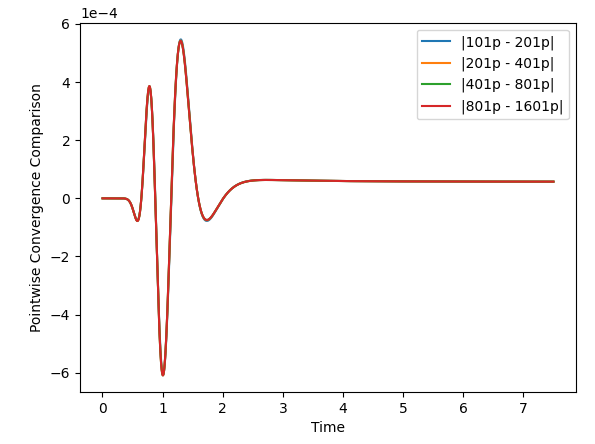
\includegraphics[width=\textwidth]{Images/Wave_Equation_3+1_Spherical-Pointwise.png}
    \end{subfigure}
    \caption{Convergence tests of the obtained evolutions for the wave equation in 3+1 dimensions with spherical symmetry using hyperboloidal coordinates. On the left, we have the $L^2$ norm convergence, and on the right, we have the pointwise convergence at $\mathscr{I}$.}
    \label{fig:spherical_compact_wave_equation-2nd_order-convergence}
\end{figure}

%----------------------------------------------------------------------------------------
%	CUBIC WAVE EQUATION IN 3+1 DIMENSIONS WITH SPHERICAL SYMMETRY
%----------------------------------------------------------------------------------------

\section{Cubic Wave Equation in 3+1 Dimensions With Spherical Symmetry}
Now it is time to tackle non-linear variations of the wave equation in 3+1 dimensions with spherical symmetry. We start by writing the wave equation as
\begin{equation}
    \Box \psi \equiv - \partial_T^2 \psi + \frac{1}{R^2} \partial_R\left( R^2 \partial_R \psi\right) = \mathcal{X} \;,
\end{equation}
where $\mathcal{X}$ is the non-linear term of our equation. Doing a first order reduction followed by the coordinate change to hyperboloidal coordinates, we get
\begin{equation}
    \left\{ \begin{array}{l} 
        \partial_T \Psi = - \Pi \\ 
        \partial_T \Phi = \mathcal{B}\left((r^2 + \Omega^2)^2 \left(H' \partial_r \Phi + \partial_r\Pi\right) + H' L \Omega \left( 2r\Phi - 3 \Omega \Psi + 2 r^{-1} \Omega^2 \Phi\right)\right) + \frac{H'\sqrt{2 L}}{H'^{\,2}-1} \mathcal{X} \\
        \partial_T \Pi = \mathcal{B}\left((r^2 + \Omega^2)^2 \left(\partial_r \Phi + H' \partial_r\Pi\right) + L \Omega \left( 2r\Phi - 3 \Omega \Psi + 2 r^{-1} \Omega^2 \Phi\right)\right) + \frac{\sqrt{2 L}}{H'^{\,2}-1} \mathcal{X}
        \end{array} \right. \; ,
\end{equation}
%
where we used the previous definition for $\mathcal{B}$. We can now substitute $\mathcal{X} = (\Psi /\chi)^3$ to obtain the cubic wave equation. 

Differently from the linear case, where we expect gaussian initial conditions that only differ by amplitude to behave similarly, in the non linear case, we expect that parameter to highly influence the solution. We will investigate this by solving the cubic wave equation with different initial conditions and comparing the results. Solving the cubic wave equation using the same boundary conditions as in the linear case, and using the initial conditions

\begin{equation}
    \begin{array}{c c c c}
        \psi(0,r) = A \, e^{-C \, r^2/2} \; , & \Phi(0,r) = - A \,C \, r \, \frac{\Omega^2(r)}{L(r)} \, e^{-C \, r^2/2} & \text{and} & \Pi(0,r) = 0
    \end{array} \; ,
    \label{eq:cubic_wave_equation-2nd_order_initial_conditions}
\end{equation}
%
with $A = 1.0$ for one of the runs and $A = 10.0$ for the other, while keeping $C = 10$ we get the results shown in figure \ref{fig:cubic_wave_eq}. We can see that, for $A = 1$, we get a solution that behaves very similarly to the linear case, as the wave starts to disperse. Differently from the linear case however, it takes longer to disperse as there is a source term. For $A = 10$, we get a solution that grows rapidly until it explodes.

\begin{figure}[h]
    \centering
    \begin{subfigure}[b]{0.45\textwidth}
        \centering
        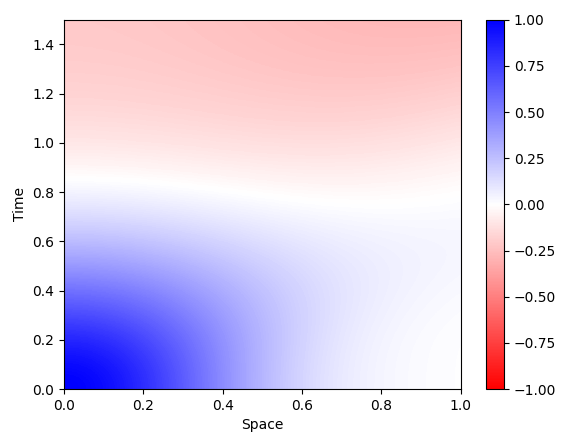
\includegraphics[width=\textwidth]{Images/Cubic_Wave_Equation_3+1_Spherical-A=1-Solution.png}
    \end{subfigure}
    \hfill
    \begin{subfigure}[b]{0.45\textwidth}
        \centering
        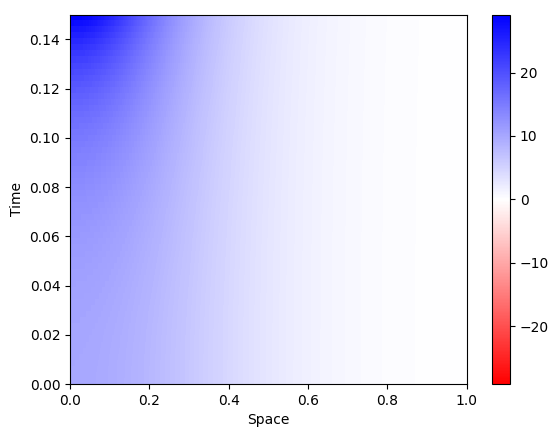
\includegraphics[width=\textwidth]{Images/Cubic_Wave_Equation_3+1_Spherical-A=10-Solution.png}
    \end{subfigure}
    \caption{Evolution of the cubic wave equation in 3+1 dimensions with spherical symmetry using hyperboloidal coordinates with the initial conditions given in equation \eqref{eq:cubic_wave_equation-2nd_order_initial_conditions}. On the left, we have $A=1$ and $C=10$. On the right, we have  $A=10$ and $C=10$.}
    \label{fig:cubic_wave_eq}
\end{figure}

Despite this rapid grouth, our solution still converges cleanly both in the norm and pointwise convergence up until the analytical blowup. This is shown in figure \ref{fig:cubic_wave_eq_convergence} for the case where $A = 10$. 

\begin{figure}[h]
    \centering
    \begin{subfigure}[b]{0.45\textwidth}
        \centering
        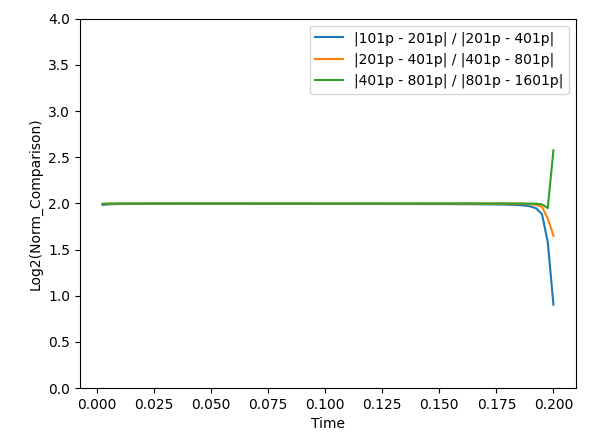
\includegraphics[width=\textwidth]{Images/Cubic_Wave_Equation_3+1_Spherical-A=10-Norm.png}
    \end{subfigure}
    \hfill
    \begin{subfigure}[b]{0.45\textwidth}
        \centering
        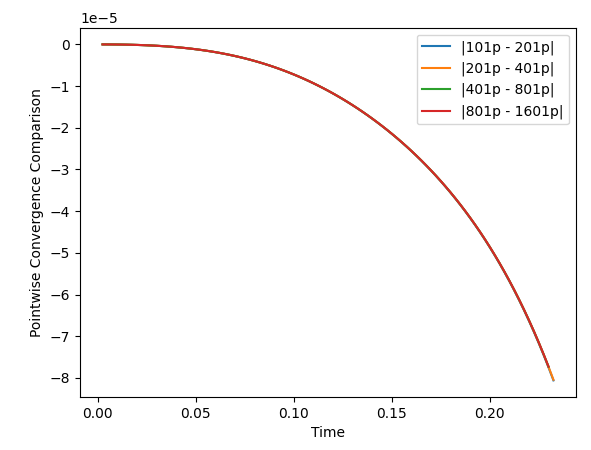
\includegraphics[width=\textwidth]{Images/Cubic_Wave_Equation_3+1_Spherical-A=10-Pointwise.png}
    \end{subfigure}
    \caption{Convergence tests of the evolution of the cubic wave equation in 3+1 dimensions with spherical symmetry using hyperboloidal coordinates, provided the initial conditions given in equation \eqref{eq:cubic_wave_equation-2nd_order_initial_conditions}, with $A=10$ and $C=10$. On the left, we have the $L^2$ norm convergence, and on the right, we have the pointwise convergence at $\mathscr{I}$.}
    \label{fig:cubic_wave_eq_convergence}
\end{figure}

%----------------------------------------------------------------------------------------
%	CONCLUSIONS
%----------------------------------------------------------------------------------------

\section{Conclusions}
Throughout this work, the hyperboloidal coordinate system proved to be a very advantageous and convenient tool when studying the behavior of outgoing waves. Our numerical experiments demonstrated the reliability of our code framework when dealing with different variations of the wave equation in these coordinates by showing clean second-order convergence in all the performed simulations.

However, this choice of coordinates is not adequate when there are incoming waves in our problem since they are very hard to resolve and are great sources of error in the simulations. This suggests that a hybrid approach may be ideal for the cases where we expect to have incoming waves in a small portion of our domain, incorporating traditional Cauchy slices alongside hyperboloidal ones.

The master thesis that follows this project will focus on expanding the well-established numerical relativity code \texttt{BAMPS}, making it able to perform simulations in this coordinate system. In addition, we will look into more intricate nonlinearities with both mathematical and physical significance such as the wave equation with quadratic nonlinearity, as we try to get closer to solving the Einstein equations numerically.

%----------------------------------------------------------------------------------------
%	BIBLIOGRAPHY
%----------------------------------------------------------------------------------------

\printbibliography[heading=secbib]

%----------------------------------------------------------------------------------------

\end{document}  
